\documentclass[main.tex,fontsize=8pt,paper=a4,paper=portrait,DIV=calc,]{scrartcl}
% Document
\usepackage[T1]{fontenc}
\usepackage[utf8]{inputenc}
\usepackage[dvipsnames]{xcolor}
\usepackage[nswissgerman,english]{babel} 
\usepackage{hyperref}
\renewcommand{\familydefault}{\sfdefault}

% Format
\usepackage[top=5mm,bottom=1mm,left=5mm,right=5mm]{geometry}
%\setlength{\headheight}{\baselineskip}
%\setlength{\headsep}{0mm}

%\usepackage{scrlayer-scrpage}
%\clearpairofpagestyles
%\chead{{\bfseries\TITLE, \AUTHOR, \pagename~\thepage}}

%\addtokomafont{pagehead}{\upshape}

\usepackage{multicol}
\setlength{\columnsep}{2mm}
\setlength{\columnseprule}{0.1pt}

% Math
\usepackage{amsmath}
\usepackage{amssymb}
\usepackage{amsfonts}

% Code
\usepackage{fancyvrb, etoolbox, listings, xcolor}
%\usemintedstyle{bw}

%\newminted[shell]{bash}{
%fontsize=\footnotesize,
%fontfamily=tt,
%breaklines=true,
%frame=single,
%framerule=0.1pt,
%framesep=2mm,
%tabsize=2
%}
%\newminted{css}{
%breaklines=true,
%tabsize=4,
%autogobble=true,
%escapeinside=||,
%stripall=true,
%stripnl=true,
%}

    \definecolor{lightgray}{rgb}{0.95, 0.95, 0.95}
    \definecolor{darkgray}{rgb}{0.4, 0.4, 0.4}
    \definecolor{purple}{rgb}{0.65, 0.12, 0.82}
    \definecolor{ocherCode}{rgb}{1, 0.5, 0} % #FF7F00 -> rgb(239, 169, 0)
    \definecolor{blueCode}{rgb}{0, 0, 0.93} % #0000EE -> rgb(0, 0, 238)
    \definecolor{greenCode}{rgb}{0, 0.6, 0} % #009900 -> rgb(0, 153, 0)
    \definecolor{teal}{rgb}{0.0, 0.5, 0.5}

\lstdefinestyle{code}{
    identifierstyle=\color{black},
    keywordstyle=\color{blue}\bfseries\small,
    ndkeywordstyle=\color{greenCode}\bfseries\small,
    stringstyle=\color{ocherCode}\ttfamily\small,
    commentstyle=\color{teal}\ttfamily\textit\small,
    basicstyle=\ttfamily\small,
    breakatwhitespace=false,         
    breaklines=true,                 
    captionpos=b,                    
    keepspaces=true,                 
    showspaces=false,                
    showstringspaces=false,
    showtabs=false,                  
    tabsize=2,
    belowskip=-5pt
}



% Images
\usepackage{graphicx}
\newcommand{\pic}{\includegraphics[scale=0.3]}
\graphicspath{{Screenshots/}{../Screenshots}}
\makeatletter
\def\pictext#1#2{%
    \@ifnextchar[{%
    \pictext@iiiii{#1}{#2}%
    }{%
      \pictext@iiiii{#1}{#2}[0.5,0.4,0.3]% Default is 5
    }%
}
\def\pictext@iiiii#1#2[#3,#4,#5]{\begin{minipage}{#3\textwidth}\includegraphics[scale=#4]{#1}\end{minipage}\begin{minipage}{#5\textwidth}#2\end{minipage}}
\def\minipg#1#2{%
    \@ifnextchar[{%
    \minipg@iiii{#1}{#2}%
    }{%
      \minipg@iiii{#1}{#2}[0.3,0.6]% Default is 5
    }%
}
\def\minipg@iiii#1#2[#3,#4]{\vspace{0.8mm}\begin{minipage}{#3\textwidth}#1\end{minipage}\begin{minipage}{#4\textwidth}#2\end{minipage}{\vspace{0.8mm}}}
\makeatother

%\newenvironment{minty}[2]% environment name
%{% begin code
%  \begin{minipage}{#1}
%  \begin{minted}{#2}
%}%
%{% end code
%  \end{minted}
%  \end{minipage}
%  \end{minty}\ignorespacesafterend
%} 

% Smaller Lists
\usepackage{enumitem}
\setlist[itemize,enumerate]{leftmargin=3mm, labelindent=0mm, labelwidth=1mm, labelsep=1mm, nosep}
\setlist[description]{leftmargin=0mm, nosep}
\setlength{\parindent}{0cm}

% Smaller Titles
\usepackage[explicit]{titlesec}

%% Color Boxes
\newcommand{\sectioncolor}[1]{\colorbox{black!60}{\parbox{0.989\linewidth}{\color{white}#1}}}
\newcommand{\subsectioncolor}[1]{\colorbox{black!50}{\parbox{0.989\linewidth}{\color{white}#1}}}
\newcommand{\subsubsectioncolor}[1]{\colorbox{black!40}{\parbox{0.989\linewidth}{\color{white}#1}}}
\newcommand{\paragraphcolor}[1]{\colorbox{black!30}{\parbox{0.989\linewidth}{\color{white}#1}}}
\newcommand{\subparagraphcolor}[1]{\colorbox{black!20}{\parbox{0.989\linewidth}{\color{white}#1}}}

%% Title Format
\titleformat{\section}{\vspace{0.5mm}\bfseries}{}{0mm}{\sectioncolor{\thesection~#1}}[{\vspace{0.5mm}}]
\titleformat{\subsection}{\vspace{0.5mm}\bfseries}{}{0mm}{\subsectioncolor{\thesubsection~#1}}[{\vspace{0.5mm}}]
\titleformat{\subsubsection}{\vspace{0.5mm}\bfseries}{}{0mm}{\subsubsectioncolor{\thesubsubsection~#1}}[{\vspace{0.5mm}}]
\titleformat{\paragraph}{\vspace{0.5mm}\bfseries}{}{0mm}{\paragraphcolor{\theparagraph~#1}}[{\vspace{0.5mm}}]
\titleformat{\subparagraph}{\vspace{0.5mm}\bfseries}{}{0mm}{\subparagraphcolor{\thesubparagraph~#1}}[{\vspace{0.5mm}}]

%% Title Spacing
\titlespacing{\section}{0mm}{0mm}{0mm}
\titlespacing{\subsection}{0mm}{0mm}{0mm}
\titlespacing{\subsubsection}{0mm}{0mm}{0mm}
\titlespacing{\paragraph}{0mm}{0mm}{0mm}
\titlespacing{\subparagraph}{0mm}{0mm}{0mm}

%% format cells
\usepackage[document]{ragged2e}
\usepackage{array, makecell}
\renewcommand{\arraystretch}{2}
\newcommand{\mc}{\makecell[{{m{1\linewidth}}}]}



\begin{document}
\tableofcontents

\newcommand{\TITLE}{Bsys2}
\newcommand{\AUTHOR}{Fabio Lenherr}
\setcounter{tocdepth}{1}

\lstset{
    language=C,
    style=code,
}

\section{C}

\subsection{fixed size types}
\begin{itemize}
\item \textcolor{purple}{int8\_t, int16\_t, int32\_t, int64\_t}\newline
  fixed integers with bit count
\item \textcolor{purple}{intmax\_t} max size int on platform
\item \textcolor{purple}{intptr\_t} signed integer with the size of an address on this platform
\item \textcolor{purple}{uint8\_t, uintptr\_t} unsigned versions
\item \textcolor{purple}{size\_t} \newline
  this is used in containers, the reson for this is that \emph{this has the max size that for example an array can be.}\newline
  \textcolor{orange}{This is unsigned!}
\end{itemize}

\subsection{Addition of pointers}
If you try to add or subtract 2 pointers to get the amount of sizeof(t) difference, then you can only do this with the exact same type, something like signed int and unsigned int will not work!\newline
\begin{lstlisting}
int32_t *y = 100;
int32_t *x = 120;
ptrdiff_t z = x - y; // z == 5
uint32_t *u = 120;  
ptrdiff_t p = u - y;  // Error: Different ptr types
\end{lstlisting}

\subsection{Index Operator on Pointers}
You can index on pointers like an array, this can be used to get elements on any object.\newline
Note that you have to manually make sure to stay within the bounds of that object, as otherwise you will have \emph{undefined behavior}.\newline
\begin{lstlisting}
int32_t x = 0;
int32_t *y = &x;
y[0] = 0x42;      // same as: x = 0x42;
(&x)[0] = 0x42;   // same
0[&x] = 0x42;     // same
100[200] = 0x42;  // Error: no address
\end{lstlisting}

\subsection{Padding}
When you mix and match different types of different sizes inside of a struct, then the compiler will include padding based on the bigger type: \newline
\begin{lstlisting}
struct  {
char c;     // Offset 0
int32_t x;  // Offset 4 --> Padding
char d;     // Offset 8
} t;        // sizeof t == 12
# structure matters!!
struct  {
char c;     // Offset 0
char d;     // Offset 1
int32_t x;  // Offset 2 --> Padding
} t;        // sizeof t == 6
\end{lstlisting}

\subsection{Forwards Declaration}
\begin{lstlisting}
struct Folder;
// Forward-Deklaration
struct File {
struct Folder *parent;
// OK: all pointer types
//
have same size
char name[256];
// OK: fixed size array
};
// --> Type complete
struct Folder {
struct File * file[256]; // OK: fixed size array
};
// --> Type complete
\end{lstlisting}

\section{Operating System APIs}

\subsection{Basic features of an Operating system}
\begin{itemize}
\item \textcolor{purple}{abstraction and portability}\newline
  \begin{itemize}
  \item \textcolor{black}{define generic APIs that work on all (as many as possible) devices}
  \item \textcolor{black}{define abstractions that we don't care about -> how are files stored on the disk?}
  \end{itemize} 
\item \textcolor{purple}{Isolation and Resource Management}\newline
  \begin{itemize}
    \item Isolate each usecase from each other -> posx
  \item \textcolor{black}{Runtime (make it blazingly fast)}
  \item \textcolor{black}{Memory Management}
  \item \textcolor{black}{Secondary Storage handling}
  \end{itemize} 
\item \textcolor{purple}{Security}
\end{itemize} 

\subsubsection{Limitations of Portability}
While the operating system can define standards, there are often things that we as developers need to consider,
for example, while the operating system can define how a user will interact with the keyboard etc, if said device \emph{doesn't have this input},
then your application will not work... Eg. An application meant for touch on the desktop might work, but not properly, and the OS can't really help there. 

\subsubsection{Limits of Isolation}
Often, you want some form of interoperability, or you are basically forced to use that.\newline
For example an application might want the focus of the keyboard, but then a popup appears.\newline
If the application continues taking the focus, then the application now breaks the user experience. 

\subsection{Processor Privilege}
Modern operating systems define a range of instructions that only the kernel is allowed to perform.\newline
This is done to protect the operating system from attacks that might be exploitable via these privlieges.\newline
\textcolor{purple}{In this case you run in \emph{user mode}}, this is also why anti-cheats are often running in kernel mode,\newline
in this mode, the anti-cheat can access any memory all the time for whatever reason the anti-cheat would like to do so. \newline
\textcolor{teal}{Should an application break the rule of user-space, the operating system will be notified and can then kill or otherwise restrict the application.}

\subsection{Kernel}
\subsubsection{MicroKernel}
\textcolor{purple}{Microkernel is the idea that only the \emph{absolutely necessary operations need to be in the kernel}, this means that often, \newline
things like drivers run in the userspace, eg. Radv would be in userspace.}\newline
Features: 
\begin{itemize}
\item \textcolor{green}{Reliability}\newline
  less code is easier to maintain, which means a more stable operating system.
\item \textcolor{green}{Analysability}\newline
  less code is easier to bisect, meaning that bug hunting is easier.
\item \textcolor{red}{Performance}\newline
  Because drivers are now in a lower priority environment, they can no longer directly access hardware.\newline
  This means that you will have a significant performance hit, which is also the reason that \emph{linux is not a microkernel!}.
\end{itemize} 
In the real world, there is no \emph{real microkernel}, they usually add the necessary functionality of drivers and leave it at that. 

\subsubsection{Monolithic Kernel}
Monolithic kernels have all the base functionality included. This means that you will not need to supply basic functionality to the kernel,\newline
just to get a functional operating system.
\begin{itemize}
\item \textcolor{green}{Performance}\newline
  Since drivers have direct access to hardware, this means they can run faster!
\item \textcolor{red}{Security}\newline
  Since drivers have direct access to hardware, this means that misconfigured or malicious hardware, \newline
  can easily infiltrate the kernel
\item \textcolor{red}{Reliablity} \newline
  More code means more possible bugs, and in the kernel this is worse than in the usermode.
\end{itemize} 

\subsubsection{Unikernel}
\textcolor{purple}{This is a kernel that is made for one specific application, which means \emph{it is an application!}.}\newline
\begin{itemize}
\item \textcolor{green}{Performance}
\item \textcolor{green}{Seurity}
\item \textcolor{green}{Reliablity}
\item \textcolor{red}{Only one Usecase}
\end{itemize} 

\subsubsection{Running an instruction in Kernel Mode}
\textcolor{purple}{When you want to run an instruction in the kernel mode, then you need to do a \emph{syscall}.\newline
The processor will then switch into kernel mode (if the os has given the privelege) and run the instruction in kernel mode.}\newline

\subsubsection{Syscall (SVC on ARM)}
\textcolor{purple}{There is only one function to run something in kernel mode, this means that we have to use \emph{codes} instead.\newline
Eg. a syscall with code 60 would be the exit code for a program. -> plox kill me}\newline
\textcolor{red}{NOTE: Syscall also doesn't take arguments, therefore you need to place the arguments in registers. \newline
This is exactly why you had to place all these things into registers, when you wanted to print a simple "hello world" in assembly. \newline
\emph{The implication: output and input are kernel mode!!}}

\subsection{ABI vs API}
\minipg{
  \textcolor{purple}{\emph{A}pplication \emph{B}inary \emph{I}nterface}
  \begin{itemize}
  \item \textcolor{teal}{concrete interfaces}
  \item \textcolor{teal}{calling conventions}
  \item \textcolor{teal}{projection of datastructures}
  \end{itemize}
}{
  \textcolor{purple}{\emph{A}pplication \emph{P}rogramming \emph{I}nterface}
  \begin{itemize}
  \item \textcolor{teal}{abstract interfaces}
  \item \textcolor{teal}{platform/OS independent aspects}
  \end{itemize} 
}[0.5,0.5]

\subsubsection{ABI in Linux}
\textcolor{purple}{Calling Conventions for syscall are different for different linux kernels!}\newline
This means that you need to compile applications for each kernel!\newline
\textcolor{purple}{To counter problems that will appear with this, there is a standard called \emph{Linux Standard Base}, which defines a set of conventions to use.}

\subsubsection{API in Linux}
\textcolor{purple}{The proper solution is to use APIs instead, which can be done with languages such as C (and tomorrow Rust).\newline
This means that you \emph{no longer use syscall}, you instead use \emph{C functions}, which work on every kernel, not just on one.}

\subsection{POSIX}
In general, every OS has its own ABI and API.\newline
\textcolor{purple}{The unix API has been developed alongside the C API, this lead to the ISO standard.}\newline
However, at some point there were multiple standards, which meant the compatability was wrecked again.\newline
\textcolor{purple}{Instead, the POSIX standard API was defined, which meant that if you wrote your program POSIX compliant, then it will run on any POSIX OS.}

\subsubsection{POSIX Conformity}
\begin{itemize}
\item \textcolor{black}{MacOS: since version 10.5}
\item \textcolor{black}{Linux, not certified, but somewhat POSIX conform}\newline
  Bad: not everything is standard, but we all know that sometimes you either go your own way, or nothing happens -> matrix
\item \textcolor{black}{Windows: no :)}
\item \textcolor{black}{BSD: yes}
\end{itemize} 

\subsection{Man Pages}
Man pages provide information about a POSIX system, it \emph{is made of 9 parts:}
\begin{enumerate}
\item \textcolor{purple}{Executable Programs or shell commands}
\item \textcolor{purple}{System calls (functions provided by the kernel)}
\item \textcolor{purple}{Library calls (functions within program libraries)}
\item \textcolor{purple}{Special files (usually fond in /dev)}
\item \textcolor{purple}{File formats and conventions, e.g. /etc/passwd}
\item \textcolor{purple}{Games lol}
\item \textcolor{purple}{Miscellaneous (including macro packages and convenstions)}
\item \textcolor{purple}{System administration commands (usually only for root)}
\item \textcolor{purple}{Kernel routines (not standard)}
\end{enumerate} 

\subsection{Shell}
\begin{itemize}
\item \textcolor{black}{Made of an ouput and input stream.}
\item \textcolor{black}{many different shells, bash, dash, zsh, fish, nu}
\item \textcolor{black}{doesn't need special rights or prerequisites}
\item \textcolor{black}{Made to call OS functions via text}
\end{itemize} 

\subsubsection{Arguments in shell}
\begin{itemize}
\item \textcolor{purple}{All arguments are considered strings -> its just an IO stream}
\item \textcolor{purple}{Spaces usually seperate the arguments}
\item \textcolor{purple}{"\textbackslash" usually used to escape characters -> like space}
\end{itemize} 
\textcolor{purple}{These arguments are then passed to C or C++ program in the array called \emph{(char **argv)}, and the \emph{(int argc)} variable is the count of arguments.}\newline
\textcolor{red}{The first entry in argv is the programname}

\subsubsection{Env Vars}
\begin{itemize}
\item \textcolor{purple}{Key-Value pair}
\item \textcolor{purple}{Example: MOZ\_ENABLE\_WAYLAND=1}
\item \textcolor{purple}{can be set for the shell in .zshrc/.bashrc etc}
\item \textcolor{purple}{can be set for environment in xdg-config/environment.d, /etc/environment or .profile, /etc/profile}
\item \textcolor{purple}{Order is root first then local, if variable is set twice, then you will overwrite it!}
\end{itemize}

\textcolor{red}{To use variables in C: getenv, putenv, setenv, unsetenv}\newline
Technically, there is a variable called \emph{environ}, which is an array of null pointers to strings which is 0 terminated.\newline
However, this variable \emph{is not defined!!} \newline
\textcolor{orange}{getenv}
\begin{lstlisting}
//definition 
char * getenv (const char * key)

char *value = getenv("PATH");
// value = "/home/ost/bin:/home/ost/.local/bin"
// returns nullptr -> 0 if variable not set
\end{lstlisting}
\textcolor{orange}{setenv}
\begin{lstlisting}
// definition 
int setenv(const char *key, const char *value, int overwrite);

int ret = setenv("HOME", "/usr/home", 1);
// returns code 0 if ok, error code otherwise 
// sets variable with value, overwrite if not 0
// error if variable doesn't exist!
\end{lstlisting}
\textcolor{orange}{unsetenv}
\begin{lstlisting}
// definition
int unsetenv(const char *key);

int ret = unsetenv("HOME");
// returns 0 if ok, error code otherwise
// removes the env variable
\end{lstlisting}
\textcolor{orange}{putenv}
\begin{lstlisting}
//definition
int putenv (char * kvp)

int ret = putenv("HOME=/usr/home");
// adds env variable pair
// returns 0 if ok, error code otherwise
// if variable already exists -> overwrite
\end{lstlisting}

\textcolor{teal}{In general, use env vars as a flag to configure things, not as a config that you \emph{need} to configure.}\newline
For other operating systems this is done via other management solutions like windows -> registry.... haah get shit on windoof users

\section{Filesystems}
\textcolor{purple}{Essentially an API that makes sure that applications do not need to understand/know how the hardware works}

\subsection{Files}
Files have 2 parts: 
\begin{itemize}
\item \textcolor{purple}{Data}\newline
  Sequence of bytes that represent the file
\item \textcolor{purple}{Metadata}\newline
  visible for users: size, date, owner, filetype hint\newline
  not visible for users: place on hardware, connection of blocks on hardware
\end{itemize} 

\subsubsection{FileTypes}
\begin{itemize}
\item \textcolor{black}{ending after . -> .pdf}
\item \textcolor{black}{File-endings have pretty much no point, they are just for the user}
\item \textcolor{black}{File-endings are used as a hint to open said file with a specific program}
\item \textcolor{black}{Type can be deducted via \emph{magic numbers} inside of the file}
\end{itemize} 
\textcolor{purple}{General Advice:}
\begin{itemize}
\item \textcolor{teal}{Data is trash unless proven otherwise}
\item \textcolor{teal}{Validate ALL data}
\item \textcolor{purple}{General advice: when decoding a file, continuously check if the file is really a pdf, or whatever you expect, test it to be. \newline
A few lines may not be enough to prove that it really is of said type.}
\end{itemize} 

\subsection{Directories}
\begin{itemize}
\item \textcolor{purple}{Essentially a file with a special type}
\item \textcolor{purple}{Each directory other than root directory has exactly one parent -> tree}
\item \textcolor{purple}{root directory is often / -> penguinOS}
\end{itemize} 

\subsubsection{Special directories}
\begin{itemize}
\item \textcolor{black}{. -> reference on self}
\item \textcolor{black}{.. -> parent reference}\newline
  for root this would just be itself..
\item \textcolor{black}{\$PWD -> working directory. getcwd in C}
\item \textcolor{black}{chdir / fchdir -> cd in C}
\end{itemize} 
Example for getting the current working directory in C:
\begin{lstlisting}
int main (int argc, char** argv) {
  char *wd = malloc (PATH_MAX);
  getcwd (wd, PATH_MAX);
  printf ("Current WD is %s", wd);
  free (wd);
  return 0;
}
\end{lstlisting}

\subsubsection{Paths}
\begin{itemize}
\item \textcolor{purple}{absolute path /home/dashie/../dashie/.zshrc}\newline
  The reason for the .. in the middle is that a canonical path is an absolute path, but without either .. or . in the middle.
\item \textcolor{purple}{relative path ../ai-app/ai-app.tex}
\item \textcolor{purple}{canonical path /home/dashie/.zshrc}\newline
  can be received with "realpath".
\end{itemize}

\subsubsection{Max Path}
\textcolor{purple}{POSIX systems can have different max path lengths, these are defined in "limits.h".}\newline
Macros: 
\begin{itemize}
\item \textcolor{purple}{NAME\_MAX} max length of filename (exclusive 0 termination)
\item \textcolor{purple}{PATH\_MAX} max length of path (inclusive 0 termination)
\item \textcolor{purple}{\_POSIX\_NAME\_MAX} minimal value of NAME\_MAX according to posix
\item \textcolor{purple}{\_POSIX\_PATH\_MAX} minimal value of PATH\_MAX according to posix
\end{itemize} 

\subsubsection{Rights}
\textcolor{purple}{There are 3 permission categories, each having 3 groups, \emph{read-write-execute} with \emph{owner-group-other}}\newline
Technically there is one more bit, the sticky bit, but this is not really used anymore.\newline
\textcolor{purple}{110-110-110 -> owner and group can do all, other can't do anything}\newline
\textcolor{teal}{Note that this can also be done with numbers -> 7 would be all -> 111}\newline
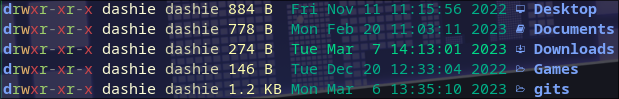
\includegraphics[scale=0.4]{2023_03_07_05_32_03.png}\newline
\textcolor{purple}{These rights are also stored as Macros in POSIX -> "sys/stat.h"}\newline
These can be chained with | -> S\_IRWXU | S\_IRGRP

\section{File API}
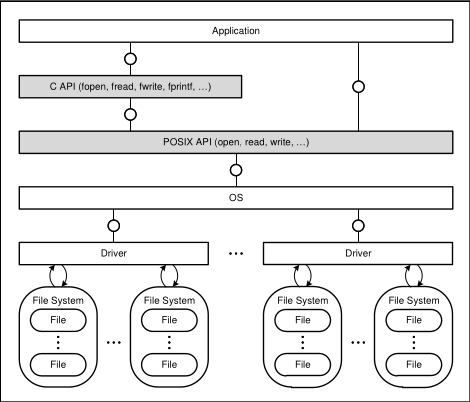
\includegraphics[scale=0.4]{2023_03_07_05_43_05.png}
\textcolor{purple}{The main difference with the POSIX API to the C API, is that the POSIX API gives us raw data, without any interpretation of the data, while the C API supports more specific things such as sockets, decoding etc.}

\subsection{POSIX File API}
General Info:
\begin{itemize}
\item \textcolor{purple}{All file functions are declared in <unistd.h> and <fcntl.h>}
\item \textcolor{purple}{error codes can be checked with "errno"}
\item \textcolor{purple}{raw data}
\item \textcolor{purple}{should only be used for binary data, not for anything that needs interpretation}
\end{itemize} 

\subsubsection{Usage of errno}
\begin{lstlisting}
if (chdir("docs") < 0) { // type is int
  if (errno == EACCESS) { // EACCESS defined in the function documentation
    printf ("Error: %s\n", strerror (errno));
    // or you can use perror
    perror ("Error"); // this makes use of the standard error stream
  }
}
\end{lstlisting}
Note, not all function set this flag, and should be used immediately, as other function will overwrite it.\newline
\textcolor{teal}{Codes for the error are directly defined in the function documentation.}\newline
\textcolor{purple}{Returns the address of a string, which describes the code in text.}\newline
perror is the same as strerror but with a special error stream.

\subsubsection{File-Descriptor}
\begin{itemize}
\item \textcolor{purple}{valid within a process}
\item \textcolor{purple}{indexed in a table of all open files in a process}
\item \textcolor{purple}{Process file table is indexed in the global table of all open files}
\item \textcolor{purple}{Receives data in order to identify physical file (correct hardware with correct driver)}
\item \textcolor{purple}{State defined: knows current offset (offset of byte that will be read next)}
\end{itemize} 
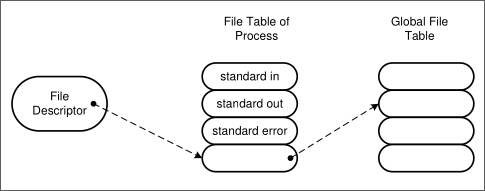
\includegraphics[scale=0.4]{2023_03_07_06_03_34.png}\newline
\textcolor{purple}{In each process open file index for a process there are 3 predefined file descriptors}\newline
\begin{lstlisting}
// STDIN_FILENO = 0  -> standard input
// STDOUT_FILENO = 1 -> standard output
// STDERR_FILENO = 2 -> standard error
\end{lstlisting}

\subsubsection{Opening files with POSIX API}
\begin{lstlisting}
int open (char *path, int flags, ...)
\end{lstlisting}
\begin{itemize}
\item \textcolor{black}{O\_RDONLY:} Read only
\item \textcolor{black}{O\_RDWR:} read and write
\item \textcolor{black}{O\_CREAT:} create file if not exists, needs another parameter for access rights
\item \textcolor{black}{O\_APPEND:} set offset to end of file before each write access
\item O\_TRUNC: set length of file to 0
\end{itemize} 

\subsubsection{Close files with POSIX API}
\begin{lstlisting}
int close(int fd)
\end{lstlisting}
deallocates file descriptor fd, which can now be used by other functions.\newline
returns 0 if ok, and -1 for error

\subsubsection{Usage of open and close}
\begin{lstlisting}
int fd = open("filename.file", O\_RDONLY);
if (fd < 0) {
  // le error handling
}
// do something with file
close(df);
\end{lstlisting}

\subsubsection{Read data with POSIX API}
\begin{lstlisting}
ssize_t read (int fd, void *buffer, size_t n)
// ssize_t is a signed size_t
\end{lstlisting}
\begin{itemize}
  \item tries to copy the next n(parameter) bytes to current offset from fd to the buffer 
\item returns count of read bytes or -1 when error
\item blocks thread until: n bytes are copied, error occurs, end of file has been reached
\item increments offset of fd by the amount of read bytes
\end{itemize} 

\subsubsection{Write data with POSIX API}
\begin{lstlisting}
ssize_t write (int fd, void *buffer, size_t n)
// ssize_t is a signed size_t
\end{lstlisting}
\begin{itemize}
  \item tries to copy the n bytes from the buffer to the offset on fd 
\item returns count of written bytes or -1 on error
\item blocks thread until n bytes are written, error occurs, or the end of file has been reached
\item increments offset of fd by the amount of bytes written
\end{itemize} 
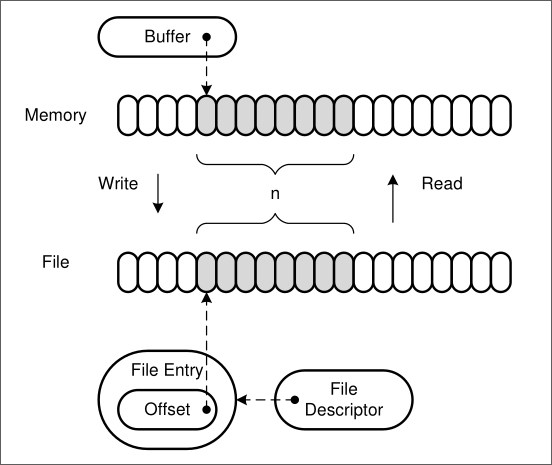
\includegraphics[scale=0.4]{2023_03_07_06_18_08.png}

\subsubsection{Jump in a file with POSIX API}
\begin{lstlisting}
off_t lseek (int fd, off_t offset, int origin)
\end{lstlisting}
\begin{itemize}
\item parameter offset that should be the new offset of fd
\item origin = SEEK\_SET for start of file
\item origin = SEEK\_CUR for current offset
\item origin = SEEK\_END for end of file
\item returns new offset or -1 on error
\end{itemize} 
Example usage:
\begin{lstlisting}
lseek (fd, 0, SEEK_CUR) return current offset
lseek (fd, 0, SEEK_END) return size of file
lseek (fd, n, SEEK_END) go beyond end of file, which will make write put 0s in this space if called. 
\end{lstlisting}
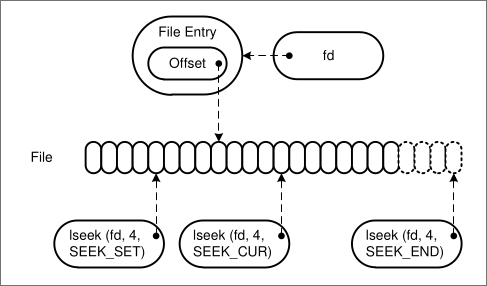
\includegraphics[scale=0.4]{2023_03_07_06_22_16.png}

\subsubsection{pread and pwrite in POSIX API}
\begin{lstlisting}
ssize_t pread (int fd, void *buffer, size_t n, off_t offset)
ssize_t pwrite (int fd, void *buffer, size_t n, off_t offset)
\end{lstlisting}
\textcolor{purple}{These are alternatives to write and read, that do not change the offset, however, this means that you will need to define where we are currently!}

\subsubsection{windoof proprietary paths}
\begin{itemize}
  \item \textbackslash instead of / because fuck you
  \item \textbackslash also needs to be escaped if you want to write it
\item root directory per disk instead of per system
\item C is the default disk, A and B were reserved for floppy disks
\item functions in windoof: \newline
  \begin{itemize}
  \item \textcolor{black}{open -> CreateFile}
  \item \textcolor{black}{read -> ReadFile}
  \item \textcolor{black}{write -> WriteFile}
  \item \textcolor{black}{lseek -> SetFilePointer}
  \item close -> CloseHandle
  \end{itemize} 
\end{itemize} 

\subsubsection{Example for reading and writing data in POSIX API}
\begin{lstlisting}
#define N 32
char buf[N];
char spath[PATH_MAX];
char dpath[PATH_MAX];

/* get paths from somewhere */

int src = open(spath, O_RDONLY);
int dst = open(dpath, O_WRONLY | O_CREAT, S_IRWXU);
ssize_t read_bytes = read(src, buf, N);
write(dst, buf, read_bytes);
close(src);
close(dst);
\end{lstlisting}

\subsection{C Stream API}
Idea: Operating systems do things differently, even something as simple as a newline is handled differently, so we need an API that can translate this to the correct symbol:\newline
\begin{lstlisting}
// Windows: \r \n = 13d 10d = 0Dh 0Ah
// Linux: \n = 10d = 0Ah
// Mac OS: \r = 13d = 0Dh (before Mac OSX, now just like penguinOS)
\end{lstlisting}
\begin{itemize}
\item \textcolor{purple}{OS independent}
\item \textcolor{purple}{stream-based: symbol-oriented}
\item \textcolor{purple}{can be buffered or unbuffered}\newline
  dependent on the implementation, transparent for applications
\item \textcolor{purple}{normally buffered for files}\newline
  independently transfers data-blocks between files and buffers
\item \textcolor{purple}{Has a file Position indicator}\newline
  - for buffered streams: defines position in buffer\newline
  - for unbuffered streams: is the offset in the file-descriptor
\end{itemize} 

\subsubsection{FILE datastructure}
\begin{itemize}
\item \textcolor{purple}{has information about a stream}
\item \textcolor{purple}{should not be used directly, instead only per pointers that are created via the C-API}
\item \textcolor{purple}{should not be copied, pointer can be used as ID by the API}
\item \textcolor{purple}{three predefined standard-streams}\newline
  \begin{itemize}
  \item \textcolor{black}{FILE *stdin}
  \item \textcolor{black}{FILE *stdout}
  \item \textcolor{black}{FILE *stderr}
  \end{itemize} 
\end{itemize} 

\subsubsection{open file with C-API}
\begin{lstlisting}
FILE * fopen (char const *path, char const *mode)
// flags
// "r": like O_RDONLY
// "w": like O_WRONLY | O_CREAT | O_TRUNC
// "a": like O_WRONLY | O_CREAT | O_APPEND
// "r+": like O_RDWR
// "w+": like O_RDWR | O_CREAT | O_TRUNC
// "a+": like O_RDWR | O_CREAT | O_APPEND
\end{lstlisting}
\begin{itemize}
\item \textcolor{black}{creates FILE-Object and stream for the file}
\item \textcolor{black}{returns pointer to created FILE-Object or 0 on error}
\end{itemize}

\subsubsection{close file with C-API}
\begin{lstlisting}
int fclose (FILE *file)
\end{lstlisting}
\begin{itemize}
\item \textcolor{black}{calls fflush}
\item \textcolor{black}{closes stream defined by file parameter}
\item \textcolor{black}{removes file from memory}
\item \textcolor{black}{returns 0 when ok, otherwise EOF}
\end{itemize} 

\subsubsection{flush of file with C-API}
\begin{lstlisting}
int fflush (FILE *file)
\end{lstlisting}
\begin{itemize}
\item \textcolor{black}{writes content to write from memory into file (if content exists)}
\item \textcolor{black}{will automatically be called when the buffer is full or file is closed}
\item \textcolor{black}{returns 0 when of, otherwise EOF}
\end{itemize} 

\subsubsection{Conversion from POSIX-API to C-API}
\begin{lstlisting}
FILE * fdopen (int fd, char const *mode)
// like fopen, but instead of path, we use a file descriptor

int fileno (FILE *stream)
// returns file-descriptor for the stream, or -1 on error
\end{lstlisting}

\subsubsection{read from file with C-API}
\begin{lstlisting}
int fgetc (FILE *stream)
\end{lstlisting}
\begin{itemize}
  \item \textcolor{black}{reads the next byte from stream \emph{as unsigned char} and returns it as int}
\item \textcolor{black}{increments the file-position indicator by 1}
\end{itemize} 
\begin{lstlisting}
char * fgets (char *buf, int n, FILE *stream)
\end{lstlisting}
\begin{itemize}
\item \textcolor{black}{reads to n-1 symbols from stream, or until newline or EOF}
\item \textcolor{black}{adds a 0 and creates a null terminated string}
\item \textcolor{black}{returns buffer(string) or 0 on error}
\item \textcolor{black}{increments the file-position indicator by the amount of read symbols}
\end{itemize} 

\subsubsection{"un"read from file with C-API}
\begin{lstlisting}
int ungetc (int c, FILE *stream)
\end{lstlisting}
\begin{itemize}
  \item \textcolor{black}{puts c(parameter -> file-descriptor) back to the stream into a special \emph{unget stack}}
\item \textcolor{black}{the next fget call will prefer the symbols in the unget stack}
\item \textcolor{black}{no change in the file itself}
\item \textcolor{black}{unget stack has a minimum size of 1 -> works at least once, can work multiple times depending on implementation}
\item returns c(parameter -> file-descriptor) or EOF on error
\end{itemize} 
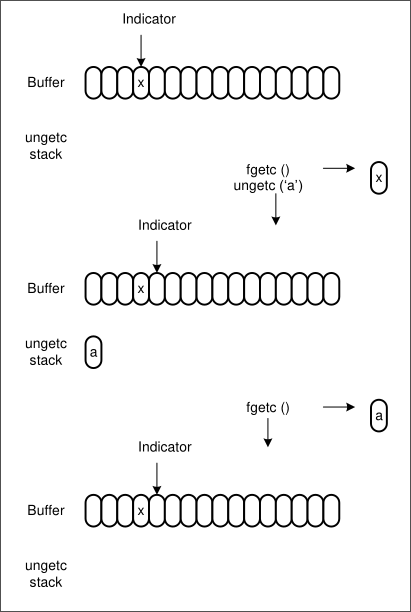
\includegraphics[scale=0.4]{2023_03_07_07_10_15.png}

\subsubsection{Write to file with C-API}
\begin{lstlisting}
int fputc(int c, FILE *stream)
\end{lstlisting}
\begin{itemize}
\item \textcolor{black}{converts file-descriptor c in unsgined char and writes it to stream}
\item \textcolor{black}{returns either c or EOF}
\item \textcolor{black}{increments the file-position indicator by 1}
\end{itemize} 
\begin{lstlisting}
int fputs (char *s, FILE *stream)
\end{lstlisting}
\begin{itemize}
\item \textcolor{black}{writes the symbols from the string s until the 0 termination symbol into the stream}
\item \textcolor{black}{the 0 termination will not be written}
\item \textcolor{black}{returns EOF on error}
\end{itemize} 

\subsubsection{End of file and Error in File C-API}
\begin{lstlisting}
int feof (FILE *stream)
// returns 0 when end of file has NOT been reached

int ferror (FILE *stream)
// retuns 0 when NO error occurred

// Example usage:
int return_value = fgetc (stream);
if (return_value == EOF) {
  if (feof (stream) != 0) {
    /* EOF reached */
  } else if (ferror (stream) != 0) {
    /* error occurred, check errno */
  }
}
\end{lstlisting}

\subsubsection{Manipulation of file-position indicator with C-API}
\begin{lstlisting}
long ftell (FILE *stream)
// returns the current file-indicator
// POSIX extension of ftello with return type off_t

int fseek (FILE *stream, long offset, int origin)
// set the file-position indicator like lseek
// POSIX extension of fseeko with off_t as type for the offset

int rewind (FILE *stream)
// reset the stream
// equivalent to fseek(stream, 0, SEEK_SET) and clear the error state
\end{lstlisting}


\subsection{Ext2}

\subsection{Ext4}

\section{Processmodels}

\section{Communication and Synchronization}

\section{Programs and libraries}

\section{Graphical Overlays}

\end{document}
